\documentclass[a4paper,11pt]{article}
\usepackage{amsmath,amsthm,amsfonts,amssymb,amscd,amstext,vmargin,graphics,graphicx,tabularx,multicol} 
\usepackage[francais]{babel}
\usepackage[utf8]{inputenc}  
\usepackage[T1]{fontenc} 
\usepackage{pstricks-add,tikz,tkz-tab,variations}
\usepackage[autolanguage,np]{numprint} 
\usepackage{calc}

\setmarginsrb{1.5cm}{0.5cm}{1cm}{0.5cm}{0cm}{0cm}{0cm}{0cm} %Gauche, haut, droite, haut
\newcounter{numexo}
\newcommand{\exo}[1]{\stepcounter{numexo}\noindent{\bf Exercice~\thenumexo} : \marginpar{\hfill /#1}}
\reversemarginpar

\newcommand{\bmul}[1]{\begin{multicols}{#1}}
\newcommand{\emul}{\end{multicols}}

\newcounter{enumtabi}
\newcounter{enumtaba}
\newcommand{\q}{\stepcounter{enumtabi} \theenumtabi.  }
\newcommand{\qa}{\stepcounter{enumtaba} (\alph{enumtaba}) }
\newcommand{\initq}{\setcounter{enumtabi}{0}}
\newcommand{\initqa}{\setcounter{enumtaba}{0}}

\newcommand{\be}{\begin{enumerate}}
\newcommand{\ee}{\end{enumerate}}
\newcommand{\bi}{\begin{itemize}}
\newcommand{\ei}{\end{itemize}}
\newcommand{\bp}{\begin{pspicture*}}
\newcommand{\ep}{\end{pspicture*}}
\newcommand{\bt}{\begin{tabular}}
\newcommand{\et}{\end{tabular}}
\renewcommand{\tabularxcolumn}[1]{>{\centering}m{#1}} %(colonne m{} centrée, au lieu de p par défault) 
\newcommand{\tnl}{\tabularnewline}

\newcommand{\trait}{\noindent \rule{\linewidth}{0.2mm}}
\newcommand{\hs}[1]{\hspace{#1}}
\newcommand{\vs}[1]{\vspace{#1}}

\newcommand{\N}{\mathbb{N}}
\newcommand{\Z}{\mathbb{Z}}
\newcommand{\R}{\mathbb{R}}
\newcommand{\C}{\mathbb{C}}
\newcommand{\Dcal}{\mathcal{D}}
\newcommand{\Ccal}{\mathcal{C}}
\newcommand{\mc}{\mathcal}

\newcommand{\vect}[1]{\overrightarrow{#1}}
\newcommand{\ds}{\displaystyle}
\newcommand{\eq}{\quad \Leftrightarrow \quad}
\newcommand{\vecti}{\vec{\imath}}
\newcommand{\vectj}{\vec{\jmath}}
\newcommand{\Oij}{(O;\vec{\imath}, \vec{\jmath})}
\newcommand{\OIJ}{(O;I,J)}


\newcommand{\reponse}[1][1]{%
\multido{}{#1}{\makebox[\linewidth]{\rule[0pt]{0pt}{20pt}\dotfill}
}}

\newcommand{\titre}[5] 
% #1: titre #2: haut gauche #3: bas gauche #4: haut droite #5: bas droite
{
\noindent #2 \hfill #4 \\
#3 \hfill #5

\vspace{-1.6cm}

\begin{center}\rule{6cm}{0.5mm}\end{center}
\vspace{0.2cm}
\begin{center}{\large{\textbf{#1}}}\end{center}
\begin{center}\rule{6cm}{0.5mm}\end{center}
}



\begin{document}
\pagestyle{empty}
\titre{Interrogation sur la symétrie axiale}{Nom :}{Prénom :}{Classe :}{Date}

\vspace*{0.5cm}


\begin{flushleft}
\begin{tabular}{|m{6cm}|m{2.5cm}|m{2.5cm}|m{2.5cm}|m{2.5cm}|}
\hline 
\textbf{Compétences} & \begin{center}
\textbf{Très bonne maîtrise}
\end{center} & \begin{center}
\textbf{Maîtrise satisfaisante}
\end{center}  & \begin{center}
\textbf{Maîtrise faible}
\end{center} & \begin{center}
\textbf{Maîtrise insuffisante}
\end{center} \\ 
\hline 
Je dois savoir construire l'image d'un point, d'un segment, d'une droite par symétrie axiale &  &  & &\\
\hline
Je dois savoir construire l'image d'un cercle par symétrie axiale &  &  & & \\ 
\hline
Je dois savoir construire l'image d'une figure par symétrie axiale  &  &  &  &\\ 
\hline 

\end{tabular} 
\end{flushleft}

\vspace*{0.5cm}

\exo{1.5} Construire sur la figure ci-dessous les symétriques A', B' et C' des points A, B et C par rapport à la droite(d).

\begin{center}
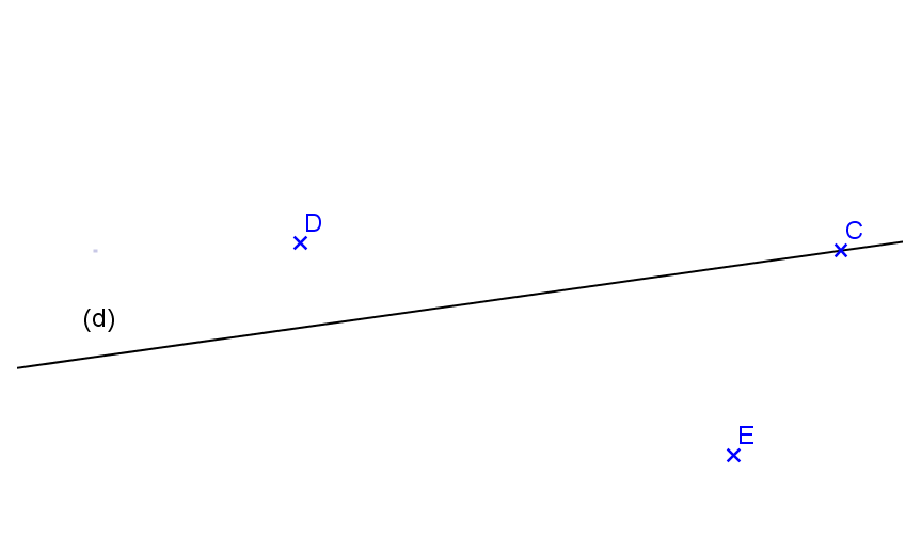
\includegraphics[scale=0.9]{interro1.eps} 
\end{center}

\exo{2.5}

\bmul{2}

Sur la figure ci-contre,\\


\qa construire les points C' et D' symétriques des points C et D par rapport à la droite $(d_{1})$ ;\\

\qa construire les points E' et F' symétriques des points E et F par rapport à la droite $(d_{2})$.\\

\columnbreak

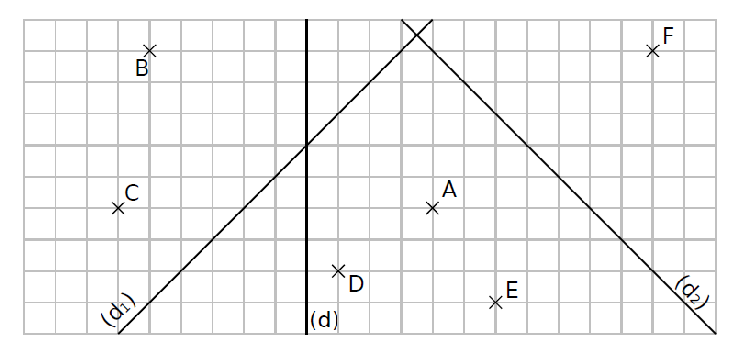
\includegraphics[scale=0.75]{interro2.eps} \\


\emul

\newpage
\vspace*{0.5cm}

\exo{2}

\begin{center}
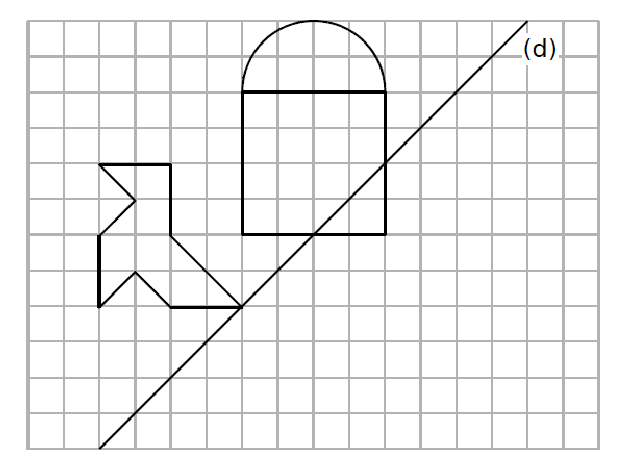
\includegraphics[scale=0.9]{interro4.eps} \\
\end{center}

\vspace*{0.75cm}

\exo{4.5}
Sur la figure suivante, tracer les symétriques par rapport à la droite (d) :\\



\initq \q du segment [DE]; \hspace*{1cm} \q du cercle (C) ;\hspace*{1cm} \q de la droite (FG) ; \hspace*{1cm}\q du triangle HIJ.\\

\begin{center}
\includegraphics[scale=0.9]{interro3.eps} 
\end{center}


\end{document}
